\documentclass[tikz]{standalone}

\begin{document}
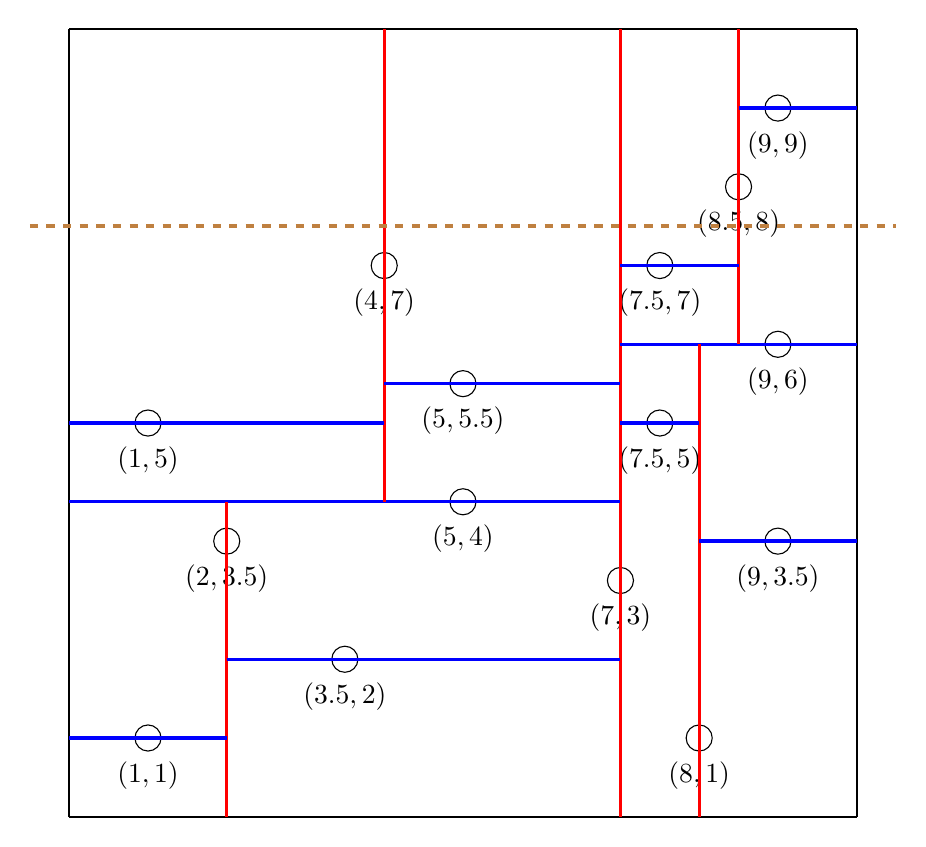
\begin{tikzpicture}[every edge/.style = {very thick, draw}]
  \draw[step = 10.0, thick] (0,0) grid (10,10);

  \foreach \p in {(1,1), (1,5), (2, 3.5), (3.5, 2), (4,7), (5, 4), (5, 5.5), 
  	(7, 3), (7.5, 5), (7.5, 7), (8,1), (8.5, 8), (9, 3.5), (9, 6), (9,9)} {
	  \node[draw, circle, minimum size = 2pt, label = {below : $\p$}] () at \p {};
  }

  \path (7,0) edge[red] (7, 10)
	(0,4) edge[blue] (7,4)
	(7,6) edge[blue] (10,6)
	(2, 0) edge[red] (2, 4)
	(4,4) edge[red] (4, 10)
	(8,0) edge[red] (8,6)
	(8.5,6) edge[red] (8.5, 10)
	(0,1) edge[blue] (2,1)
	(0,5) edge[blue] (4,5)
	(2,2) edge[blue] (7,2)
	(4, 5.5) edge[blue] (7, 5.5)
	(7,5) edge[blue] (8,5)
	(7,7) edge[blue] (8.5, 7)
	(8, 3.5) edge[blue] (10, 3.5)
	(8.5, 9) edge[blue] (10, 9);

  \draw[dashed, ultra thick, brown] (-0.5, 7.5) to (10.5, 7.5);
\end{tikzpicture}
\end{document}